\documentclass[12pt,article]{article}

\usepackage{amssymb, amsmath, amsthm} 
\usepackage{graphicx}
\usepackage{natbib}
\usepackage[dvipsnames]{xcolor}

\newcommand{\todo}[1]{\textcolor{red}{#1}}

\begin{document}

\begin{center}
\Large{\scshape Delta-bitscore for non-coding Human DNA variation} 
\end{center}

\section{Introduction}

\begin{itemize}

\item scorring methods help to identify pathotogenic genes. These methods mostly targeted coding parts of the genome. However the non-coding variation can be associated with functional consequencies. 

\item Recently, there have been developed different scorring methods for non-coding DNA. The comparison of the existing methods have been done in \citet{drubay2018benchmark}.

\item \citet{wheeler2016profile} introduced a profile-based scoring method to identify variants associated with gene function divergence. They introduced a delta-bitscore as a reflection of gene conservation and applied it to amino acid variation. 

\item We propose to use this approach for scoring non-coding DNA. We apply this method to a well characterised human non-coding DNA dataset~\citep{biggs2020ncVarDB}. 

\item We compare our method with the existing ones. 

\end{itemize}

Here, we investigated the distributions of delta-bitscores for pathogenic and benign human non-coding variants. 

\section{Materials and methods}

\subsection{Workflow} 

For each variant:

\begin{itemize}
\item retrieve the alignment of the  +/-100 nucleotide region 
\item built an HMM for the alignment
\item score the variant and reference sequences against the HMM
\item calculate delta bitscore as $x_{ref} - x_{var}$
\end{itemize}



\subsection{Dataset}

The dataset that we have previously curated \cite{biggs2020ncVarDB} consists of \todo{770} pathogenic and \todo{9240} benign variants. Each variation is represented by either a single nucleotide mutation (SNP), or an insertion or a deletion of a block of several nucleotides. Each pathogenic variant has been shown to be associated with a certain disease as described in \cite{biggs2020ncVarDB}. The set of benign variants consists of variants that occur in the population with high frequencies (over 5\%). 

\subsection{HMM models}

To build HMM models for pathogenic and benign variants we retrieved 100 way human to vertebrate alignment from UCSC dataset. Then we build the HMM from the alignments in the region corresponding to +/-100 nucleotides away from the modified region. Thus if a variation is due to a SNP then the region is 201 nucleotides long. If it is an insertion of a block of $n$ nucleotides then the region length is 200 for the reference and $200+n$ for the alternate sequence and vise versa for a deletion of an $n$-nucleotide block. We treated a duplication in a similar way as an insertion when it comes to the region length. 

\section{Results}

The distributions of the delta bit-scores for pathogenic and benign variants have distinct modes~\ref{densities}. However, there is a large overlap. 

\begin{figure}
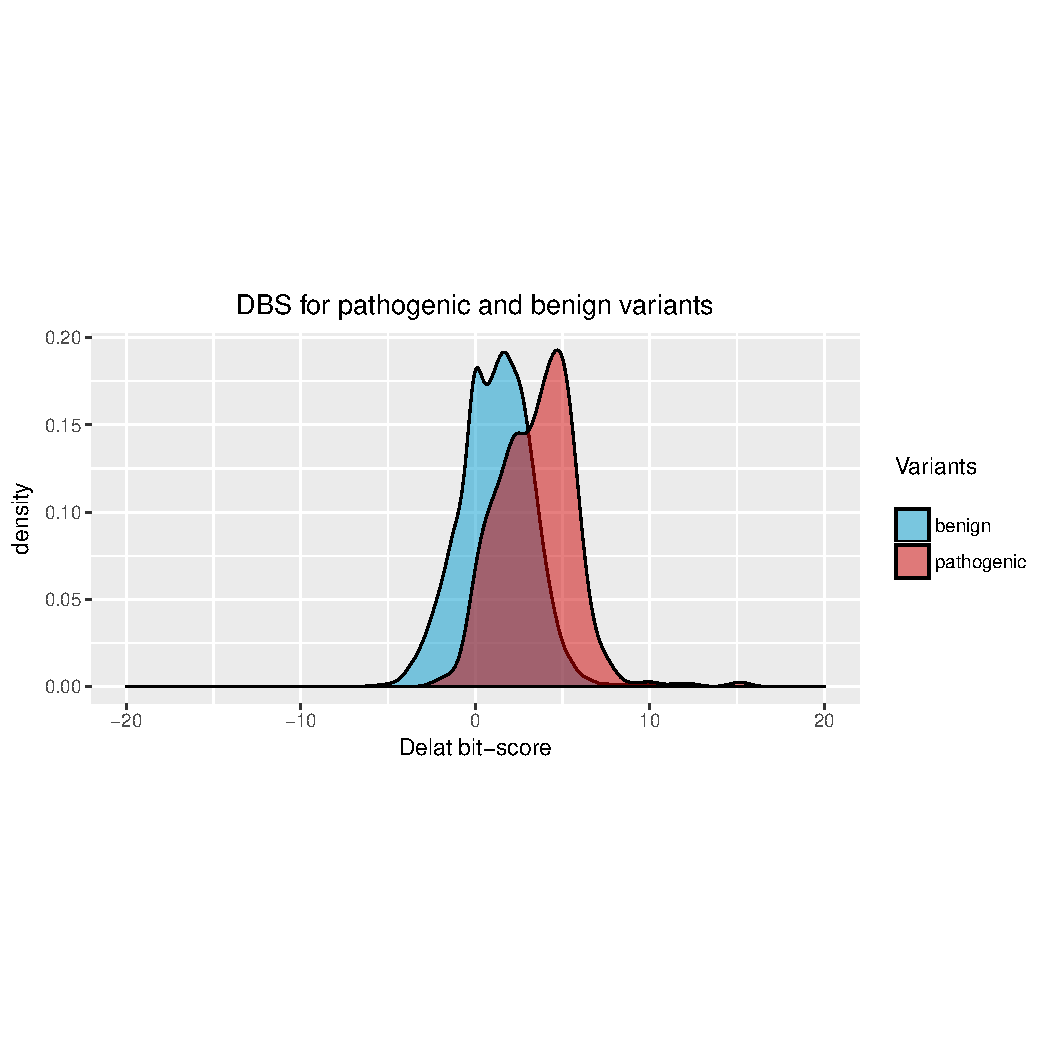
\includegraphics{../Human_Harrys_data/plots/DBscore_densities_ggplot_within20.pdf}
\label{densities}
\end{figure}

A logistic regression analysis shows that the test based on the delta bit-score has ...

\begin{figure}
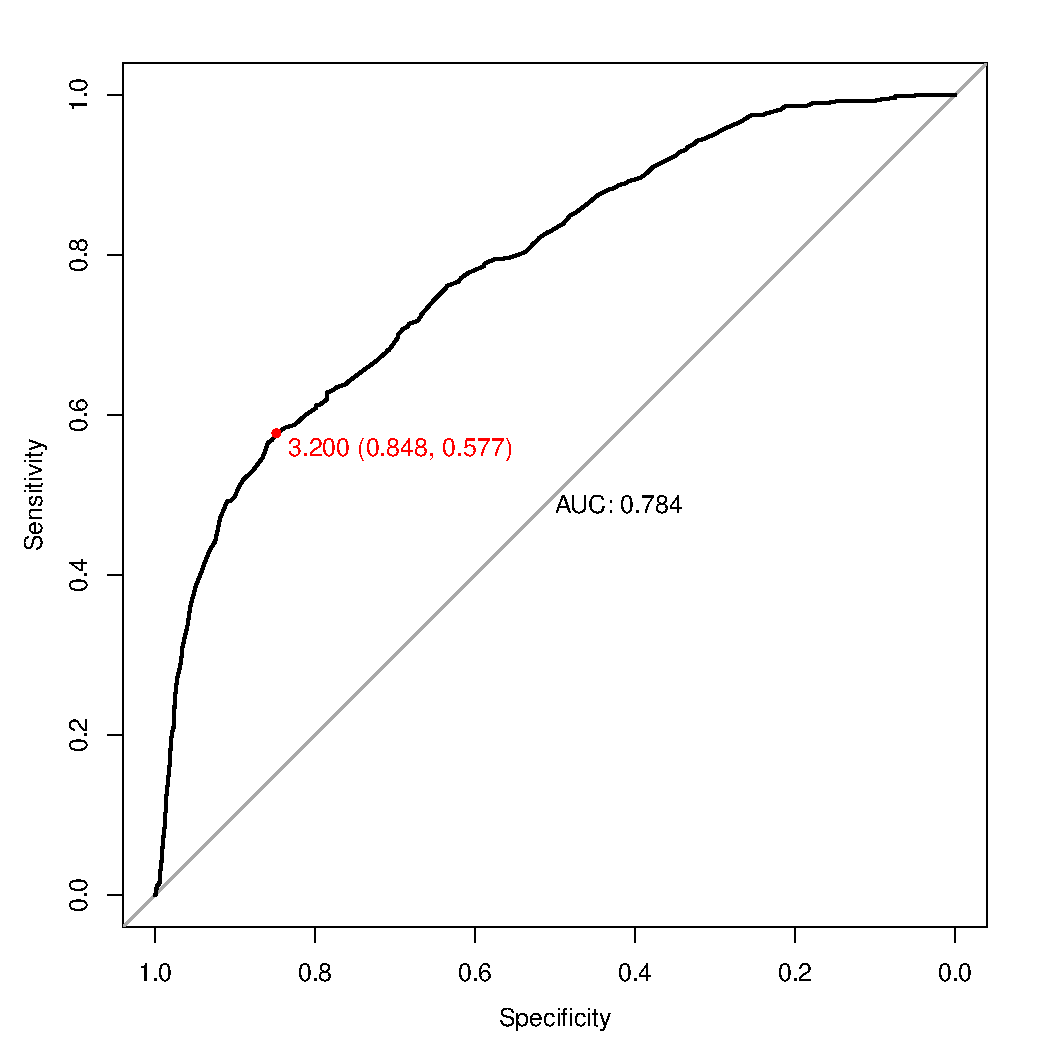
\includegraphics[width=0.5\textwidth]{../Human_Harrys_data/ROCcurve.pdf}
\end{figure}

We have found that the high absolute values of delta bit scores were associated with upstream proximity to the top predictor genes found in \citet{wheeler2018machine}. 






\section{Discussion}

\begin{itemize}
\item problem with the pathogenic dataset - association
\end{itemize}

\bibliographystyle{bevbib4} 
\bibliography{ncdbs}



\end{document}